\begin{frame}{Architectures}

  \begin{center}
    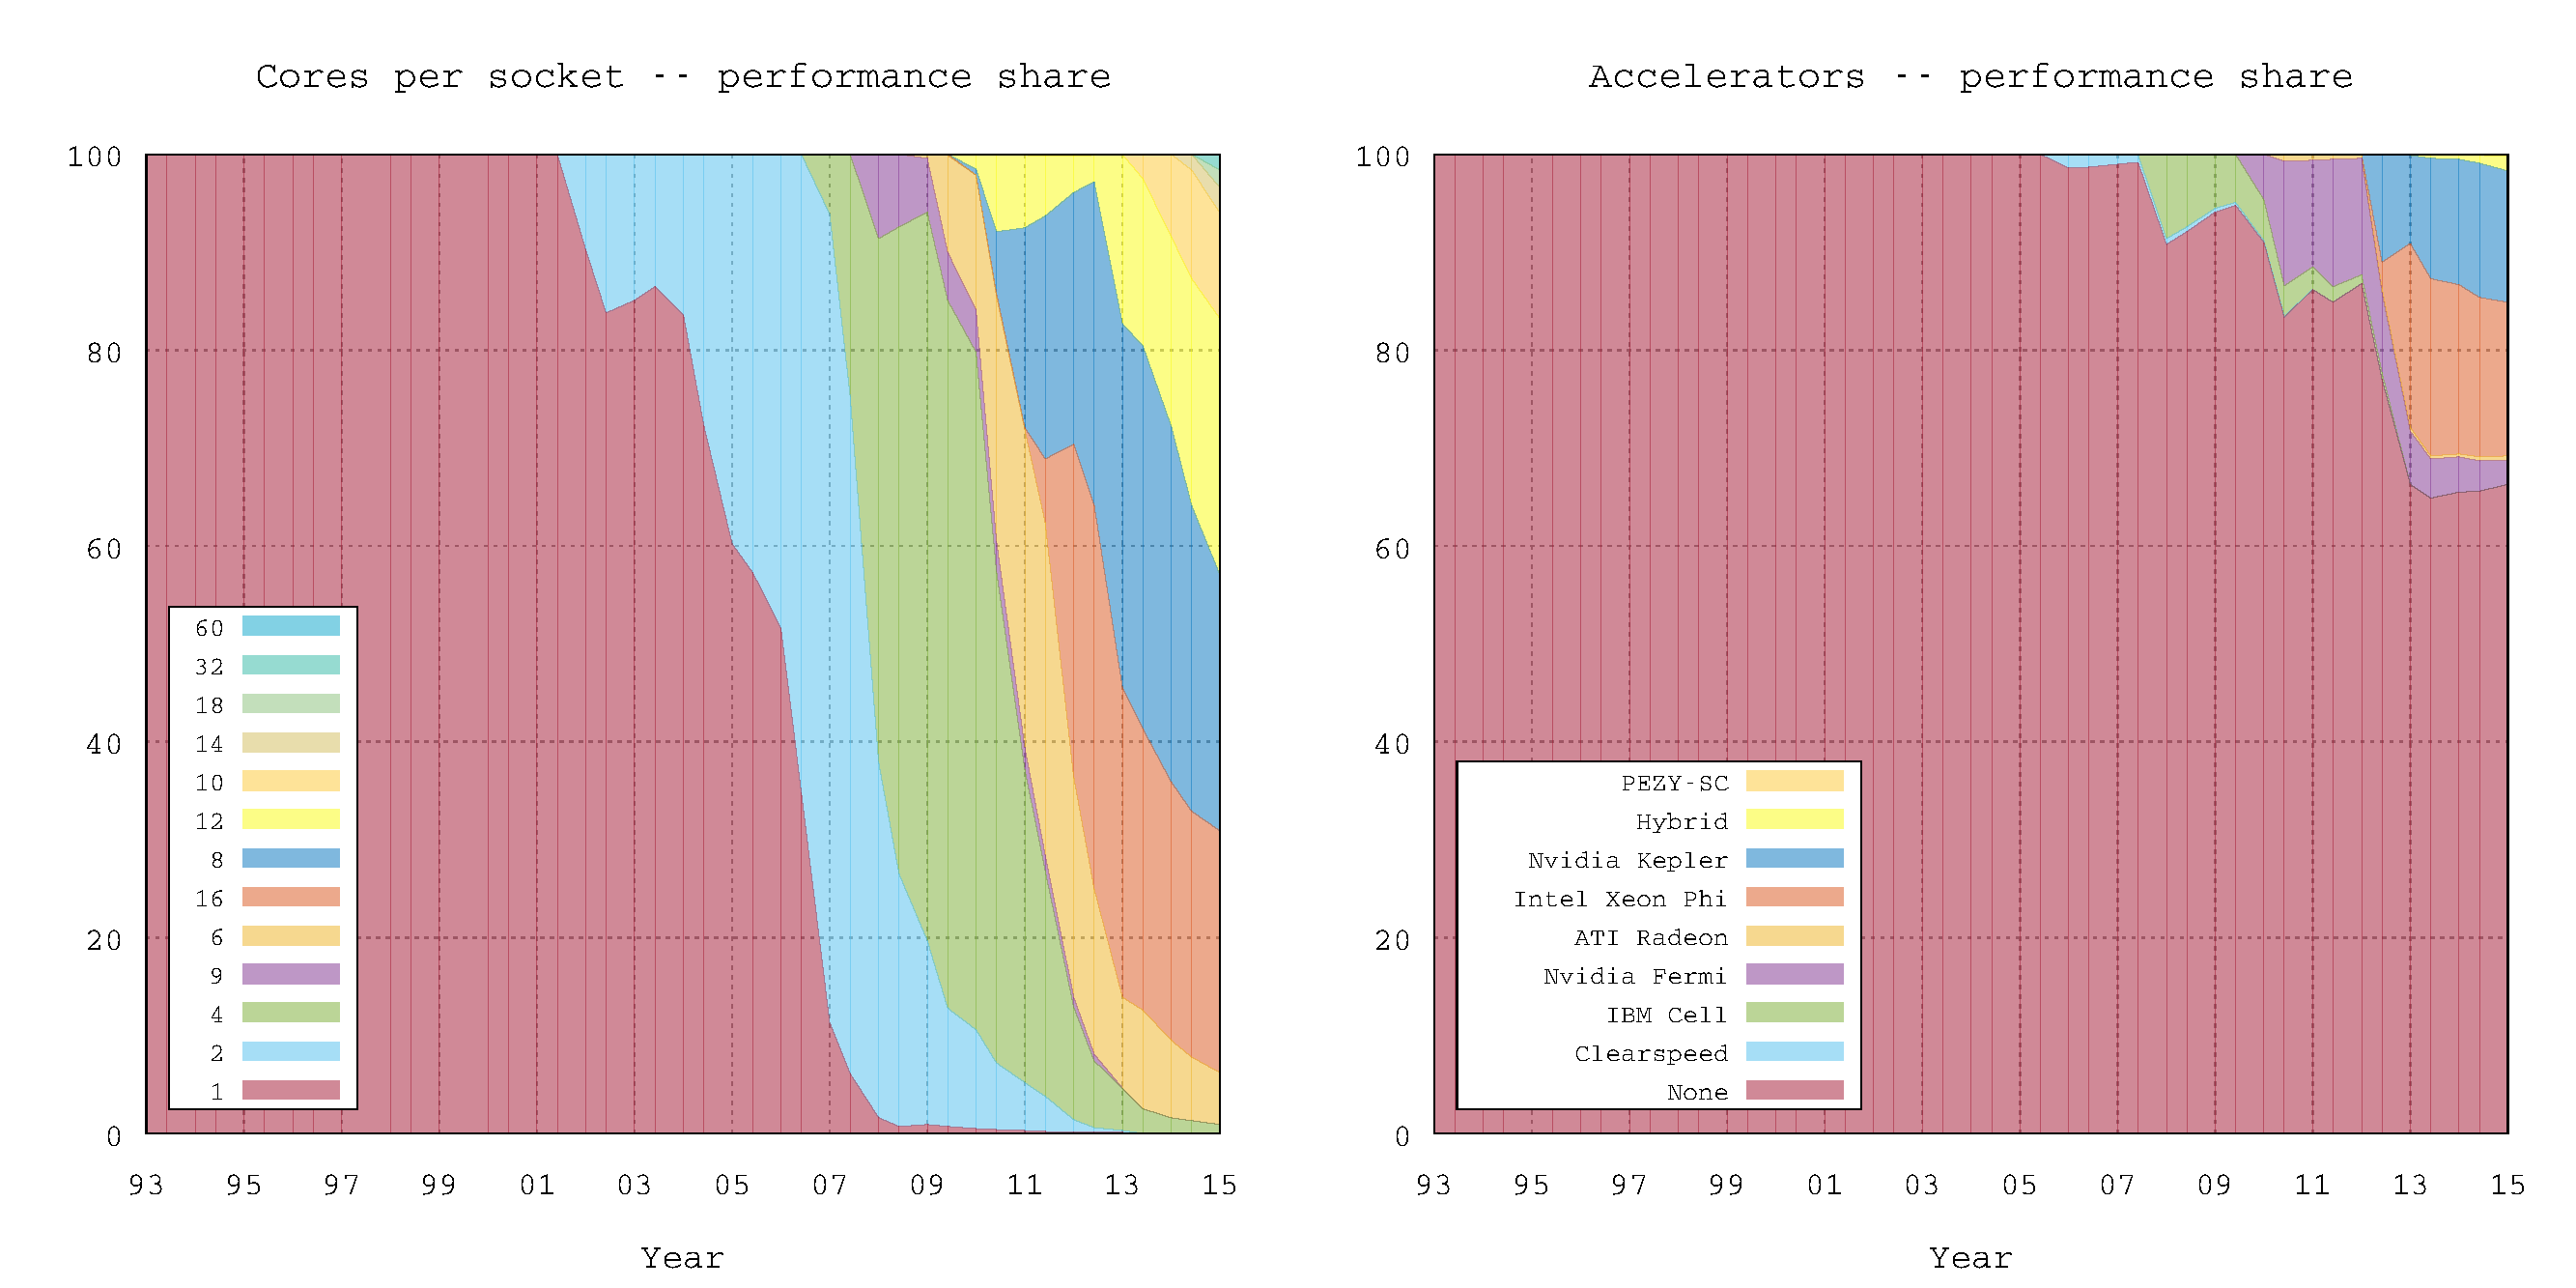
\includegraphics[width=0.9\textwidth]{data/top500}
  \end{center}

  According to the \dr{Top500 lists}, multicore
  architectures introduced in 2001 nowadays represents 100 \% of
  the performance share in the list. Accelerator, such as \db{GPU}
  and \db{Xeon Phi devices}, started gaining interests in the HPC
  community in 2005 and became very popular ever since.

\end{frame}

\begin{frame}{Tree pruning in the multifrontal method}
  The elimination tree is split in two parts using a NG\&Geist-like method:
  \begin{itemize}
  \item<2-> \dg{Top}: tree and node parallelism with hierarchical partitioning. 
  \item<4-> \db{Bottom}: sequential subtrees (only tree parallelism) with
    MAGMA-like (\alert{with staircase}), coarse-grain partitioning.
  \end{itemize}

  \vspace{0.5cm}

  \begin{center}
    \only<1>{\includegraphics[width=0.8\textwidth]{figures/lzero-0} }% 
    \only<2>{\includegraphics[width=0.8\textwidth]{figures/lzero-1} }% 
    \only<3>{\includegraphics[width=0.8\textwidth]{figures/lzero-2} }% 
    \only<4>{\includegraphics[width=0.8\textwidth]{figures/lzero-3} }% 
  \end{center}


\end{frame}

\begin{frame}{Task granularity: GPU vs CPU}
  \centering
   
  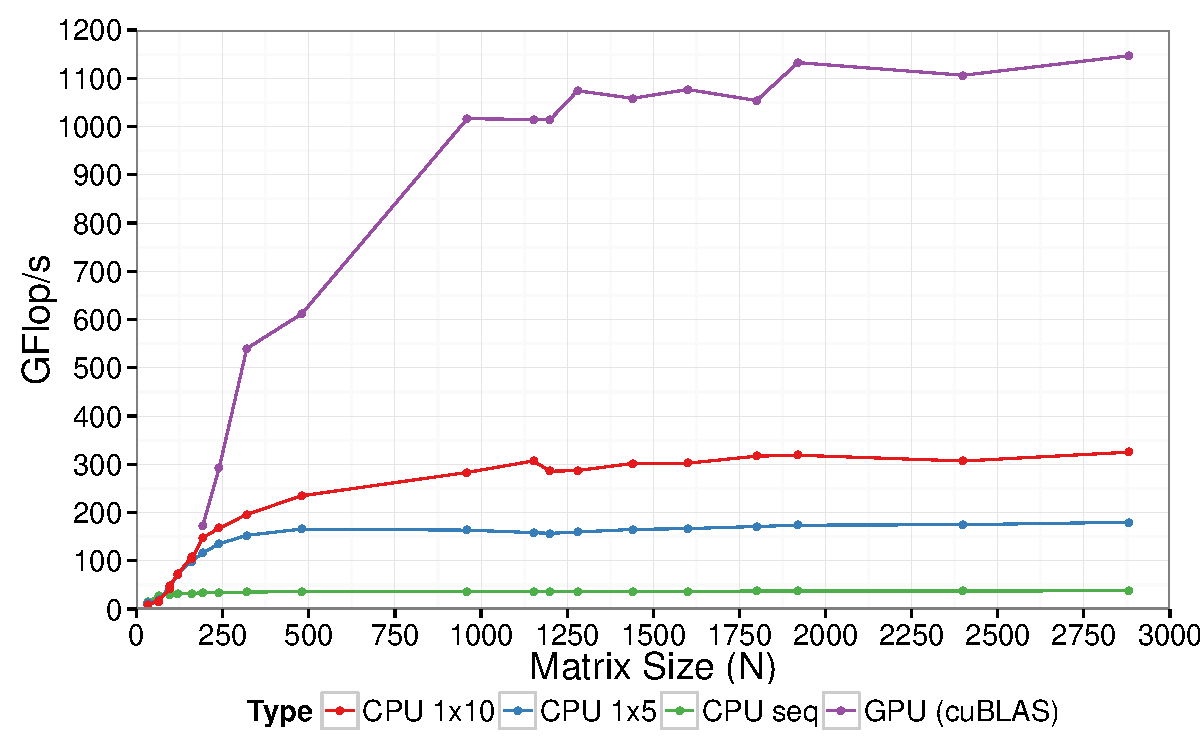
\includegraphics[width=0.9\textwidth]{figures/cholesky_GEMM_evaluation_nolog}

\end{frame}

\begin{frame}{The PTG parallel multifrontal QR factorization}
  \centering
   
  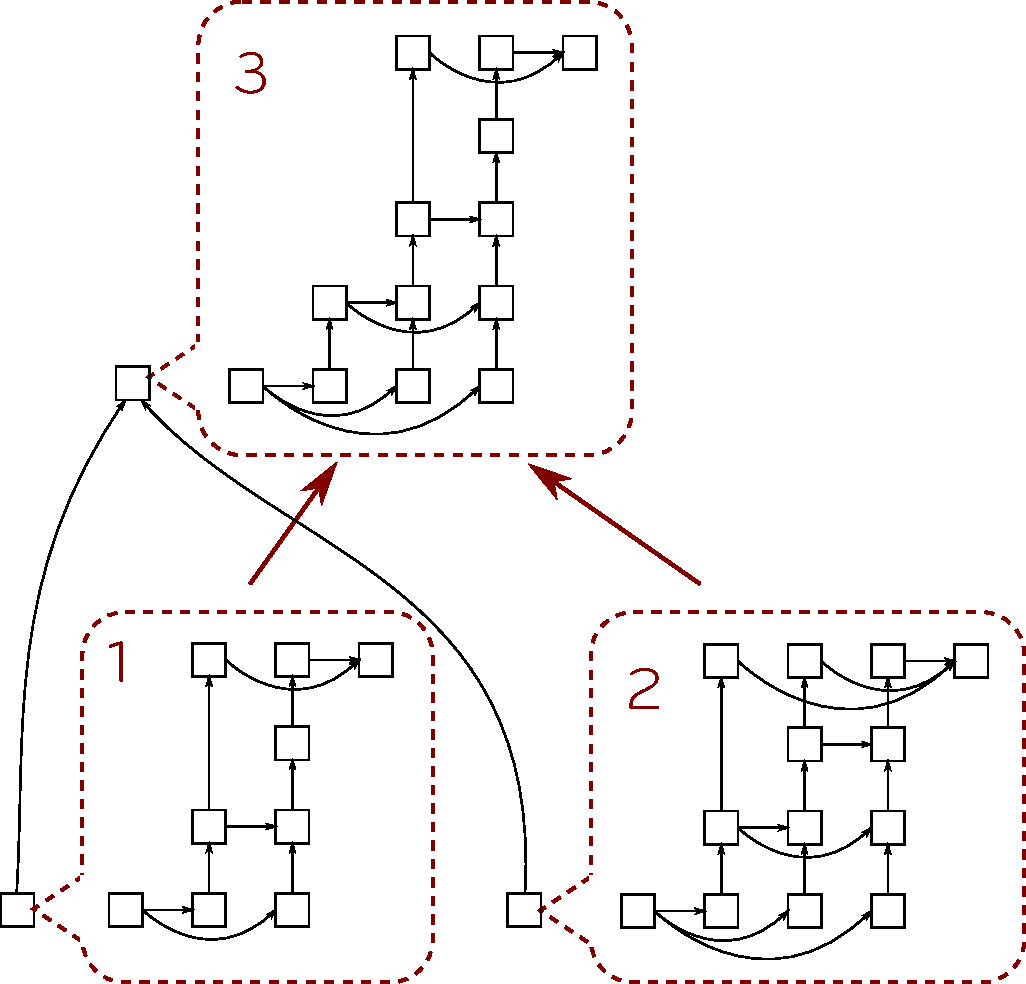
\includegraphics[width=0.4\textwidth]{figures/dag_parsec}

  Two level hierarchical DAG
  \begin{itemize}
  \item \dr{\texttt{factorization.jdf}}: the JDF representing the
    factorization DAG (Top level DAG).
  \item \dr{\texttt{qr\_1d.jdf, qr\_2d.jdf}}: the JDF files for the
    frontal matrix factorization DAGs (inner DAGs).
  \item \dr{\texttt{assembly.jdf}}: the JDF for the assembly (inner DAG)
    operations.
  \end{itemize}

\end{frame}

\begin{frame}{The PTG programming model: example}
  \begin{columns}
    \begin{column}{0.5\textwidth}    
      \lstinputlisting{listings/seq-example.c}
    \end{column}
    \begin{column}{0.5\textwidth}
      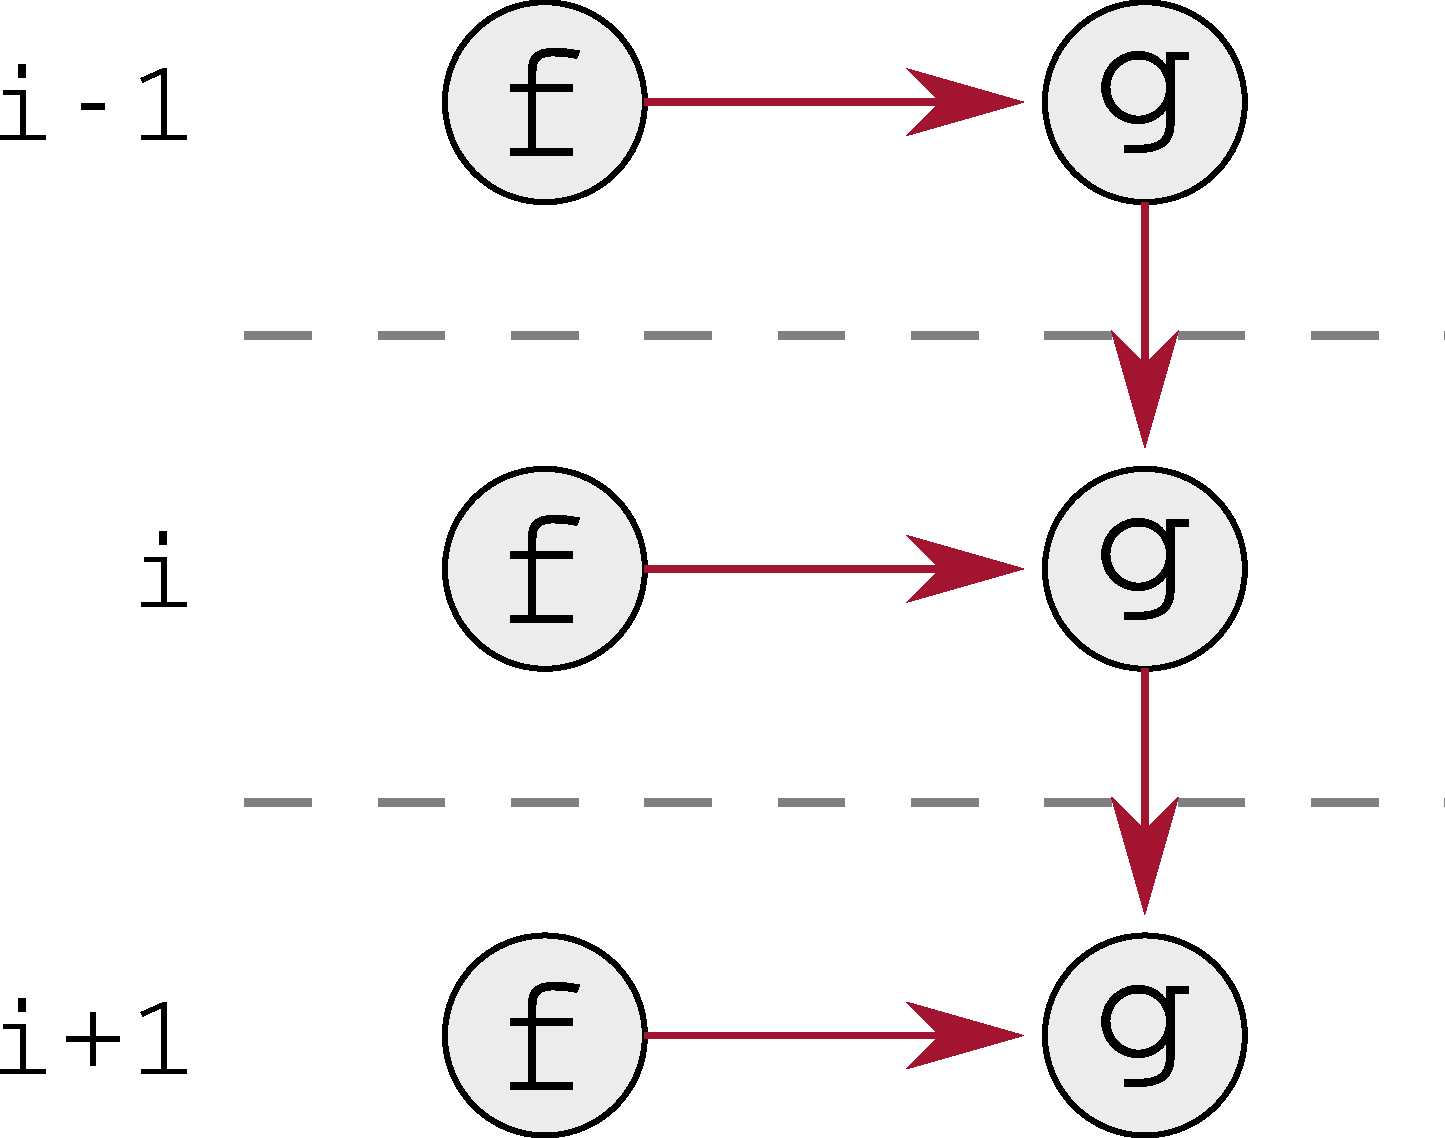
\includegraphics[width=0.7\textwidth]{figures/example_dag}
    \end{column}
  \end{columns}    
\end{frame}

\begin{frame}{The PTG programming model: example}
  \centering
  \lstinputlisting[language=C, procnamekeys={}]{listings/ptg-example.c}
\end{frame}

\begin{frame}{The PTG parallel multifrontal QR factorization}
  \centering
  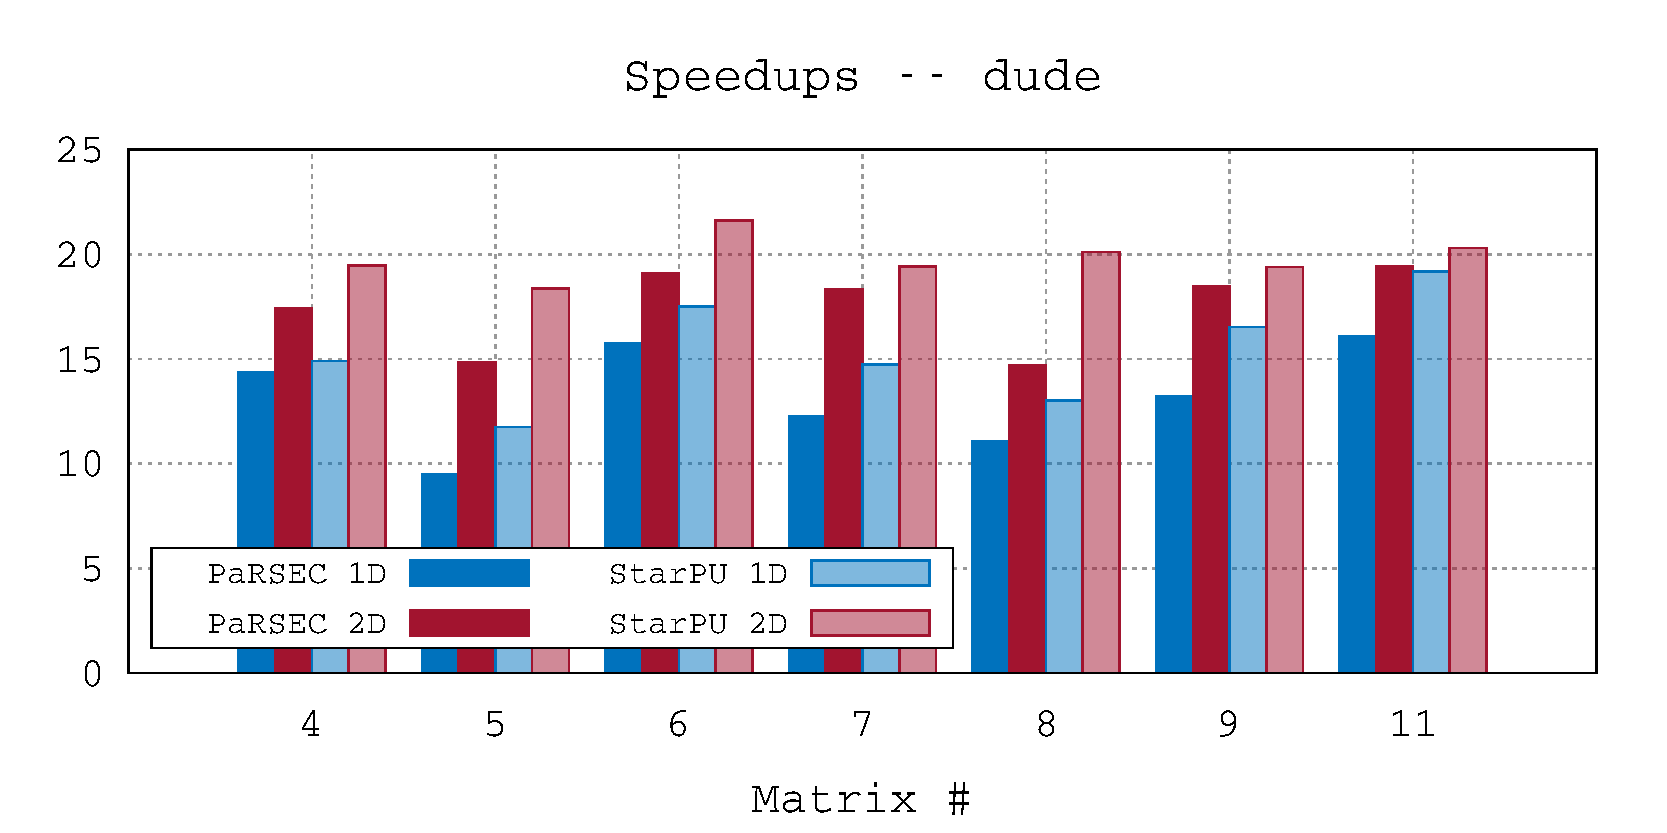
\includegraphics[width=\textwidth]{data/starpu_parsec_su}
\end{frame}

\begin{frame}{Critical path analysis}
  \centering
  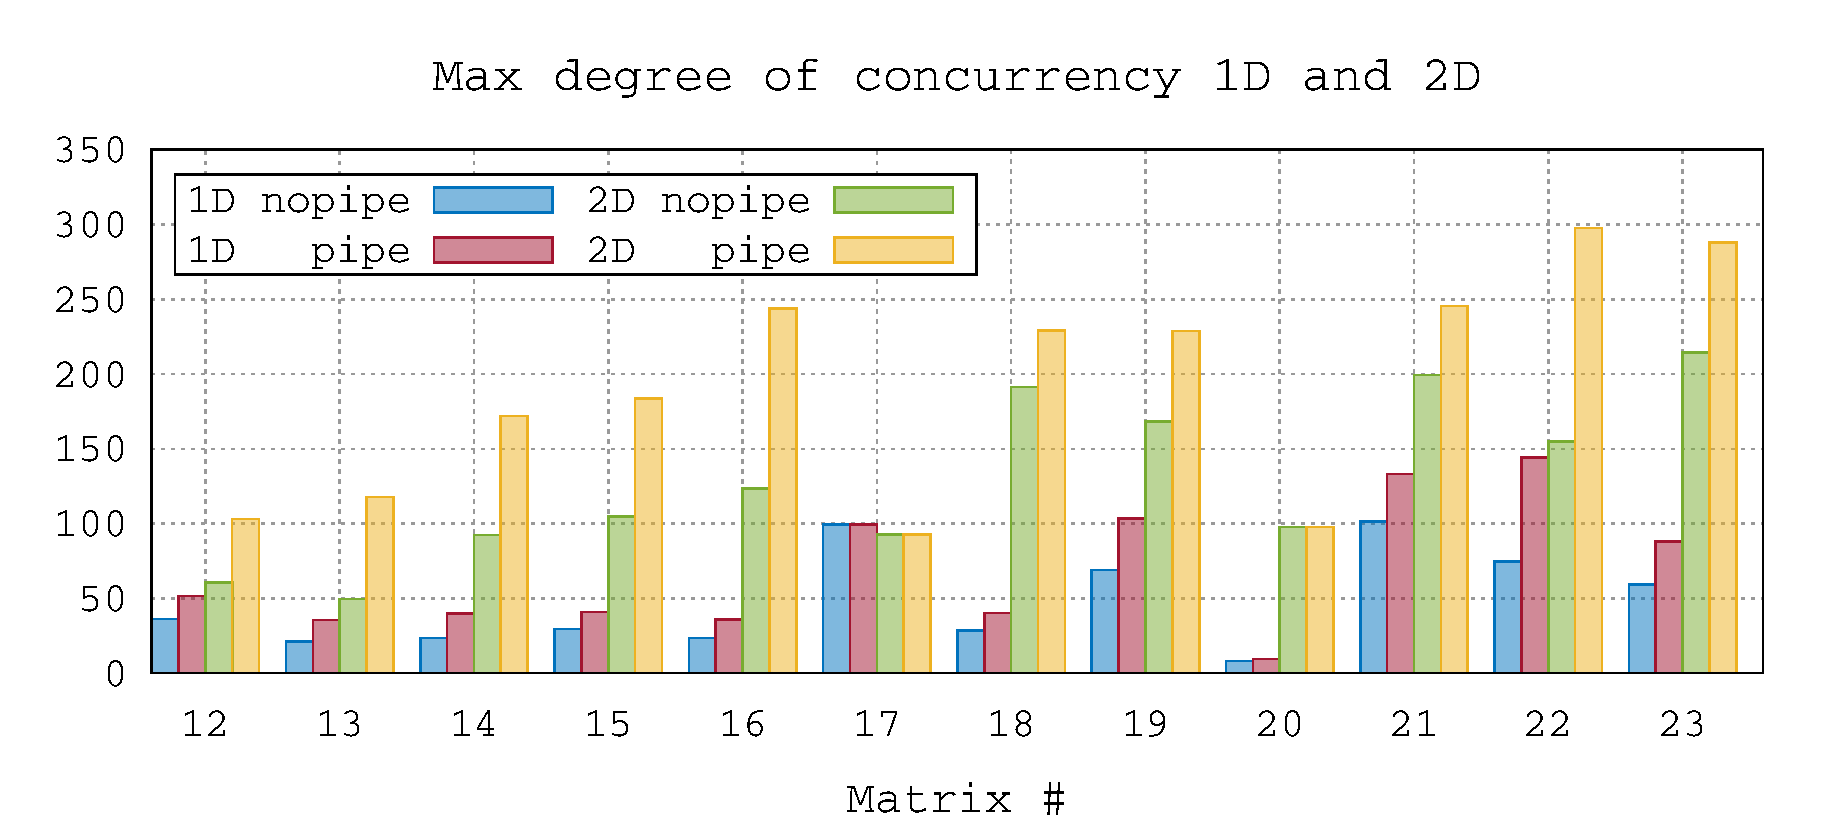
\includegraphics[width=0.9\textwidth]{data/cp_ada_toms_2d}

  \begin{displaymath}
    \text{max\_speedup}=\text{avg\_concurrency} = \frac{\sum_{i \in DAG}
      w_i}{\sum_{i \in CP} w_i}
  \end{displaymath}

  \begin{itemize}
  \item The \dr{DAG} used to conduct this analysis is the one related
    to the case where \dr{32 working threads} are used.
  \item The \dr{weight} of tasks is chosen to be equal to the
    \dr{execution time} measured in an execution with only one working
    thread.
  \end{itemize}

\end{frame}
